\chapter{Background}
\label{chap:background}

% Introduce and summarise this chapter
\section{Reinforcement Learning}
\label{sec:background:rl}

In reinforcement learning, the standard representation of an
environment and task instance is a Markov decision process (MDP). An
MDP can be represented as the tuple, $\tuple{ \states, \actions,
\transitions, \rewards, \gamma }$, where $\states$ and $\actions$ are
the state and action domains which are known to the agent.
$\transitions: \states \times \actions \to \measure(\states)$, where
$\measure(\states)$ is the set of all probability measures over
$\states$, describes the dynamics of the world through state-action
transition probabilities. $\rewards: \states \times \actions \to \Re$
describes the task at hand by ascribing rewards for state transitions.
Both $\transitions$ and $\rewards$ are initially unknown to the agent.
Finally, $\gamma \in [0,1)$ is a parameter, called the `discount
factor', that weighs the value of future rewards. 

\begin{figure}[ht]
  \centering
  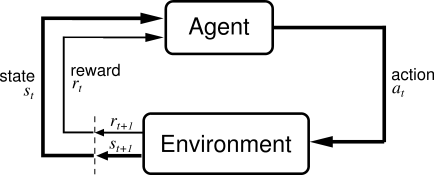
\includegraphics[width=3in]{figures/agent-environment.png}
  \caption{Agent-Environment Interface}
  \label{fig:agent-env}
\end{figure}

% Figure here
In this setting, an agent in a state $s \in \states$ chooses an action
$a \in \actions$, and moves to a state $s'$ with probability
$\transitions(s'|s,a)$, receiving a reward $\rewards(s,a)$
(\autoref{fig:agent-env}). In the fully observable setting, the agent is
aware of which state it is in, and the objective of the agent is to find
a policy $\policy: \states \to \measure( \actions )$, i.e. a decision
procedure for selecting actions, that maximises the reward it
accumulates in the long run, $R = \sum_{i} \gamma^i r_i$. $R$ is also
called the return. 

In the remainder of this section, we will describe the basic approach
for finding an optimal policy $\policy$ for a discrete MDP, and its
continuous variant. 

% Various representations of MDPs

% Discrete MDPs
\subsection{Discrete Markov Decision Processes}
 
In the discrete case, $\states$ and $\actions$ are predictably finite
sets of states and actions. We define the value function $V^{\pi}:
\states \to \Re = \E_{\pi}[\sum_{t=0}^{\infty} \gamma^{t} R_t | S_0
= s ]$ to be the expected return from $s$, and $Q^{\pi}: \states \times
\actions \to \Re = \E_{\pi}[\sum_{t=0}^{\infty} \gamma^{t} R_t | S_0
= s, A_0 = a ]$ to be the expected return from $s$, after taking the
action $a$. These can be written in a recursive form,
\begin{eqnarray*}
  V^{\pi}(s) &=& \max_{a} \rewards(s,a) + \gamma \sum_{s' \in \states} \transitions(s'|s,a) V^{\pi}(s') \\
  Q^{\pi}(s,a) &=& \rewards(s,a) + \gamma \sum_{s' \in \states} \transitions(s'|s,a) Q^{\pi}(s',a').
\end{eqnarray*}

Our objective can then be stated as finding a policy $\pi$ with an
optimal value function, i.e. $V^{*}(s) = \sup_{\pi} V^{\pi}(s)$ at all
$s \in \states$. The optimal value functions must satisfy the Bellman
optimality conditions, 
\begin{eqnarray*}
  V^{*}(s) &=& \max_{a} \rewards(s,a) + \gamma \sum_{s' \in \states} \transitions(s'|s, a) V^{*}(s') \\
  Q^{*}(s,a) &=& \rewards(s,a) + \gamma \sum_{s' \in \states} \transitions(s'|s,a) \max_{a'} Q^{*}(s',a').
\end{eqnarray*}

Given an optimal $Q$, it is possible to construct a greedy policy that
is optimal; $\pi(s,a^*) = 1$ when $a^* = \argmax_{a} Q(s,a)$, and $0$
otherwise. In principle, if the agent knew the MDP, it could construct
the optimal value function, and from it an optimal policy.  However,
in the typical setting, the agent is only aware of the state-action
space, $\states$ and $\actions$, and must learn $Q$ through
exploration. The Q-learning algorithm learns $Q$ with a simple update
for every step the agent takes, $$Q(s,a) = Q(s,a) + \alpha
[ r + \gamma \max_{a'} Q(s',a') - Q(s,a) ],$$ where $\alpha \in [0,1]$
is a parameter that controls the learning rate.  It has been shown
that the Q-learning algorithm converges to the optimal value function
in the limit with fairly permissive assumptions.

% Continuous MDPs
\subsection{Continuous Markov Decision Processes} 

In continuous domains, defining $\states$ and $\actions$ must be done
with some care. To begin with, $\states$ must be a measurable
Euclidean space \footnote{Roughly, a space $X$ is said to be
measurable if a monotonic function $\mu: 2^X \to \Re$ that is additive
over finite union can be defined.}; let us denote the Lebesgue measure
\footnote{The Lebesgue measure is a generalisation of length/area. It
is possible to construct a Lebesgue measure for any Euclidean space.}
by $\lambda$.  Consider the following (mild) regularity assumption
proposed in \citet{Andra2008}, 
\begin{property}(MDP Regularity)
  \label{prop:mdp-regularity}
  $\states$ is a compact subset of the $d_{\states}$-dimensional
  Euclidean space, $\actions$ is a compact subset of $[-A_{\infty},
  A_{\infty}]^{d_{\actions}}$. The random immediate rewards are bounded
  by $\hat{R}_{\max}$ and $\rewards$ is uniformly bounded by $R_{\max}:
  \|r\|_{\infty} \le R_{\max}$.
\end{property}

We define the evaluation operator; $T^{\pi}:B(\states \times \actions)
\to B(\states \times \actions)$, $$ T^{\pi}Q(s,a) = \rewards(s,a)
+ \gamma \int_{\states,\actions} \ud s' \ud a'~ \transitions(\ud
s'|s,a) \pi(a'|s') Q(s',a').  $$ We now define the analogue of the
$Q$-value function recurrence relation, $Q^{\pi} = T^{\pi}Q^{\pi}$.
The fixed point of the Bellman operator $T :B(\states \times \actions)
\to B(\states \times \actions)$, $$ TQ(s,a) = \rewards(s,a) + \gamma
\int_{\states} \ud s'~ \sup_{a' \in \actions} \transitions(\ud s'|s,a)
Q(s',a'),$$ $Q^* = TQ^*$ is then the optimal value function. By the
regularity conditions imposed in \autoref{prop:mdp-regularity},
$V^{\pi}$ and $Q^{\pi}$ are both bounded by $\frac{R_{\max}}{1
- \gamma}$.

In order to approach learning an optimal policy, we must estimate the
current value function, $Q$. One method is to use a function
approximator. Another popular scheme is the Fitted Q-iteration
approach, wherein the $Q$ function is estimated by regressing on
a finite trajectory collected using a stationary policy $\pi_b$. Let
$[S_t, A_t, R_t]_{1 \le t \le N}$, be the dataset, and then $Q_{k+1}$
can be got by, $$Q_{k+1} = \textrm{Regress}( \left\{ [(S_t, A_t), R_t
+ \gamma \max_{a' \in \actions} Q_k(X_{t+1},a')]_{1 \le t \le N-1}
\right\} ).$$

The regression itself can be solved using a variety of methods,
including neural networks and SVMs. A further discussion on suitable
regression methods, and a proof of convergence subject to niceness
assumptions can be found in \citet{Andra2008}.

\section{Spatial Abstractions: Homomorphisms}
\label{sec:background:homs}

% TODO: Clean up.
A homomorphism is defined in general to be a structure-preserving map.
In the context of MDPs, we want a correspondence between the two
systems' dynamics ($\transitions$) and tasks ($\rewards$). 

\begin{definition}(MDP Homomorphism)
An MDP homomorphisms $h$ from an MDP $\mdp = \tuple{S,A,P,R,\gamma}$ to
and MDP $\mdp' = \tuple{S',A',P',R',\gamma}$ is a surjection for the
state-action spaces $S \times A \to S' \times A'$ such that,
\begin{eqnarray}
  P'(h(s,a),\him{s'}) &=& \sum_{s' \in \finv{f}(\him{s'})} P(s,a,s') \label{condition:hom-P} \\
  R'(h(s,a)) &=& R(s,a), \label{condition:hom-R} 
\end{eqnarray}
\noindent
where $f$ is $h$ restricted to $S$, i.e. $f(s) = h(s,a)\mid_S$, and
$\him{s'}$ is the image of $s'$ in $\mdp'$, i.e. $\him{s'} = f(s')$.
\end{definition}

With minor abuse of notation, we assume $P(h(s,a),\him{s'}) \triangleq
P(\him{s}, \him{a}, \him{s'})$, where $h(s,a) = (\him{s}, \him{a})$.
Similarly, $Q(h(s,a)) = Q(\him{s},\him{a})$. For brevity, we will write
$\mdp \hom{h} \mdp'$ if $\mdp'$ is the homomorphic image of $\mdp$ under
$h$. We will also use the notation $(s,a) \in \mdp$ to mean $(s,a) \in
S \times A$. Finally, two state-action pairs $(s,a)$ and $(s',a')$ are
equivalent if $h(s,a) = h(s,a') = (\him{s},\him{a})$. We write this as
$(s,a) \sim (s',a')$.

There can be other, less strict definitions of homomorphisms based on
preserving the value function, policy behaviour, etc. A survey of these
definitions can be found in \cite{Li06}.

% Description of major problems for homomorphisms.
Given this definition, there are perhaps four serious questions that
we wish to answer when talking about homomorphisms,
\begin{enumerate}
  \item (Transfer) Given a homomorphisms $g$ between MDPs $M$ and $M'$,
    can one use a policy learnt in $M$ in $M'$, and vice versa?
  \item (Discovery) Given MDPs $M$ and $M'$, are they homomorphic? 
  \item (Minimisation) Given an MDP $M$, what is the smallest $M'$
    isomorphic to $M$?
  \item (Approximate Minimisation) Given an MDP $M$, and a class of
    homomorphisms $H$, what is the closest approximation $M' \in H(M)$
    of $M$?
\end{enumerate}

All of these questions have been convincingly answered in the case of
discrete MDPs. 

% Description of how homomorphisms can be used to pull back policies 
\subsection{Transferring Policies in Discrete MDPs}

The primary application of MDP homomorphisms is in the transfer of
learning in problem to another. 

\begin{definition}(Lifted Policy)
  Given $\mdp \hom{h} \mdp'$, and a policy $\pi'$ in $\mdp'$ we can
  define a {\em lifted policy} $\pi = \finv{h}(\pi')$ in $\mdp$ as
  follows,
  \begin{eqnarray}
    \pi(s,a) &\triangleq& \frac{\pi'(h(s,a))}{ |\{a':h(s,a') = h(s,a)\}| }. \\
             &=& \frac{\pi'(h(s,a))}{ |\{a':(s,a') \sim (s,a)\}| }.
  \end{eqnarray}

  Note that the denominator equally distributes the selection
  probability between equivalent actions for a state.
\end{definition}

A powerful result that we will later review shows that the lifted
policy of an optimal policy is itself optimal. This is a special case
of the result that the value of the lifted policy is equal through out
$M$ to the value of the original policy in $M'$, i.e. for all $s$,
$V^{\pi}(s) = V^{\pi'}(\him{s})$.

% Description of how homomorphisms can be used in context of relativized options.
\begin{note}(Partial Homomorphisms and Relativised Options)

  \begin{figure}[ht]
    \centering
    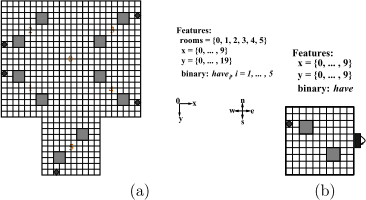
\includegraphics[width=3in]{figures/relativized-options.png}
    \caption{Relativised Options}
    \label{fig:relativised-options}
  \end{figure}

The ability to `lift' policies from one MDP to another can be exploited to
solve subproblems in a reinforcement learning domain. Consider the grid-world
shown in \autoref{fig:relativised-options}(a) taken from \cite{Ravindran2003};
in this domain, there are several rotated copies of the room shown in
\autoref{fig:relativised-options}(b). For each room in (a), let us define a
homomorphism mapping each cell within the room to those of the template room
(b). All states outside the room are mapped to the `sink' state, denoted by the
black square in (b). We can now define {\em options}
\cite{SuttonPrecupSingh1999} for each room, using the optimal policy for (b),
$\pi$, and the above homomorphisms; $\options = \{\finv{h_r}\pi(a) \mid \mbox{for
each room $r$} \}$.

\end{note}

\section{Temporal Abstractions: The Options Framework}
\label{sec:background:options}

The options framework provides a temporal abstraction through subtasks.
An option $\option$ is described by an initiation set $\initset \subset
\states$, a policy $\pi$, and a terminating condition $\beta$.  An agent
can exercise an option in any state $s \in \initset$, following which,
it will follow the policy $\pi$ described by the option, until the
terminating condition $\beta(s)$ is satisfied. The terminating condition
$\beta$ can be stochastic.

Several learning algorithms have been proposed for agents using options
\cite{SuttonPrecupSingh1999,BartoMahadevan2003}. One simple such method that
we will use is MacroQ, a generalisation of the Q-learning algorithm
described above. The MacroQ algorithm updates the value function only
after completion of the option. If the option $o$ was initiated in the
state $s$, and continues for $k$ steps before terminating in $s'$, the
corresponding $Q$ function update will be,
\begin{eqnarray*}
    Q(s,o) &=& Q(s,o) + \alpha [ r + \gamma^{k} \max_{o' \in \actions \cup \options} Q(s',o') - Q(s,o) ].
\end{eqnarray*}

Different tasks in the same domain can be described by different
$\rewards$. Let $\rewards$ be sampled from the family $\Rewards$. Our
objective then is to find a set of options $O$ that reduces the expected
learning time over $\Rewards$.

\begin{example}
  \label{example:taxi}

\begin{figure}[th]
    \centering
    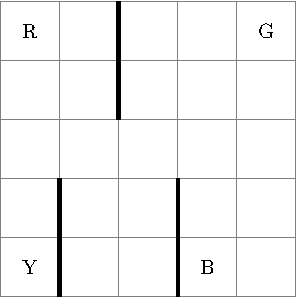
\includegraphics{figures/taxi}
    \caption{The Taxi Domain}
    \label{fig:taxi-domain}
\end{figure}
To make the discussion more tangible, let us look at an example, the
Taxi domain, shown in \figref{fig:taxi-domain}. The agent is a taxi
navigating in this road-map. It must pick up a passenger at one of the
4 pads, R, G, B or Y.  Subsequently, it must carry the passenger to a
destination, which is also one of the above four pads. The states of
the taxi would then be a tuple containing the location of the
passenger (in one of the four pads, or within the taxi), the
destination of the passenger, and location of the taxi in the map.
The actions the taxi can perform are moving up, down, left or right in
the map, as well as pick up or drop a passenger at a pad. 
Typical options for such a domain would be an option that can be
started anywhere, and has a policy that takes the taxi to the one of
the pads in the shortest possible manner. Such an option is generic,
and does not depend on where the passenger or destination are. The RL
agent must then learn to choose the right option when picking up the
passenger.
\end{example}

\section{Small World Networks}
\label{sec:background:sw}

\begin{figure}[ht]
  \centering
  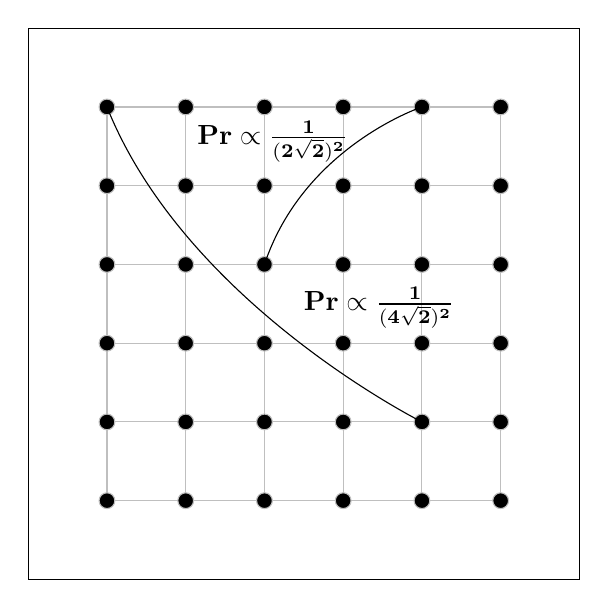
\begin{tikzpicture}[]
    % Grid
    \draw[clip] (-1,-1) rectangle (6,6);
    \draw[step=1,color=lightgray] (0,0) grid (5,5);
    \foreach \xpos in {0, 1, 2, 3, 4, 5}
    {
      \foreach \ypos in {0, 1, 2, 3, 4, 5}
      {
      \draw [color=lightgray,fill=black,opacity=1.0] (\xpos,\ypos) circle (0.1);
      };
    };

    % Draw some long range edges
   \draw (2,3)  .. controls (2.5,4.5) and (4,5) .. node [left] {$\mathbf{Pr \propto \frac{1}{(2\sqrt{2})^2}}$} (4,5);
   \draw (0,5)  .. controls (1.0,2.5) and (4,1) ..  node [above right] {$\mathbf{Pr \propto \frac{1}{(4\sqrt{2})^2}}$} (4,1);

\end{tikzpicture}
  \caption{Kleinberg's Small World Network}
  \label{fig:kleinberg-sw}
\end{figure}

% What are small world options
In Kleinberg's small-world network model (\figref{fig:kleinberg-sw}),
each node $u$ is given one `long-range' edge to a node $v$, which was
chosen with a probability $P_r(u,v) \propto \|u-v\|^{-r}$, where
$\|u-v\|$ denotes the least distance between nodes $u$ and $v$ in the
graph. On an $r$-dimensional lattice, $\klein_r$, the distance from
any node $u$ to a target node $t$ is bounded by $\|u-t\|$, a quantity
which is locally computable. When given long-range edges distributed
according to $P_r$, \citet{Kleinberg2000} showed that a greedy
distributed algorithm $\greedyalgo$ that chooses a neighbour $v$
closest to $t$ will reach $t$ with an expected time $O(\log(|V|)^2)$.
This result is significant because the expected time for the algorithm
on a graph with edges distributed uniformly, i.e. without dependence
on distance, is $O(|V|^2)$.

\begin{theorem}
  \label{thm:kleinberg-sw}
  Let $f: V \to \Re$ be a vertex function, and $M_f$ be the global
  maxima of $f$. Consider an algorithm, \greedyalgo, that greedily
  chooses the neighbour with the highest value of $f$. Suppose the
  algorithm is currently at $u$, it will choose $N(u) = \argmin_v \|f(v)
  - f(M_f)\|$.
  
  If $\graph(V,E)$ is $r$-dimensional lattice, and contains a long
  distance edge distributed according to $P_r: p(u,v) \propto
  \|u-v\|^{-r}$, then \greedyalgo takes $O( (\log |V|)^2 )$ steps to
  reach $M_f$.
\end{theorem}
\begin{proof}
  We defer the proof of this theorem to \secref{sec:sw:theory}, where we
  prove a generalisation of this theorem (\thmref{thm:sw}).
\end{proof}

